\documentclass[letterpaper,12pt]{article}

\RequirePackage{comment}
\RequirePackage[hypertex]{hyperref}
    \hypersetup{colorlinks=true,urlcolor=blue,linkcolor=red}
\RequirePackage{GE05}

\newcommand{\GDP}{\mbox{\em GDP\/}}
\newcommand{\NDP}{\mbox{\em NDP\/}}
\newcommand{\GNP}{\mbox{\em GNP\/}}
\newcommand{\NX}{\mbox{\em NX\/}}
\newcommand{\NY}{\mbox{\em NY\/}}
\newcommand{\CA}{\mbox{\em CA\/}}
\newcommand{\NFA}{\mbox{\em NFA\/}}
\newcommand{\Def}{\mbox{\em Def\/}}
\newcommand{\CPI}{\mbox{\em CPI\/}}

\def\ClassName{The Global Economy}
\def\Category{Class Notes}
\def\HeadName{Business Cycle Theory}

\begin{document}
\thispagestyle{empty}%
\Head

\centerline{\large \bf \HeadName}%
\centerline{Revised: \today}

\bigskip
We've seen that economic fluctuations follow regular patterns 
and that these patterns can be used to forecast the future.  
For some purposes that's enough.
But if we want to make sense of analyst discussions of business conditions,  
of monetary policy, 
or of situations that don't fit the historical patterns, 
we need a theoretical framework.  
%We give you two for the price of one.  
Think of these notes as the executive summary; 
textbooks devote hundreds of pages to the same topic.  


\subsubsection*{Aggregate supply}

The standard business cycle model used by journalists and analysts 
is an adaptation of the supply and demand diagram.
We refer to the curves as aggregate supply and aggregate 
demand to emphasize that we're talking about the whole economy 
rather than a single market --- 
and to remind ourselves that the analogy with supply and demand 
in a single market is imperfect.   
Figure \ref{fig:asad} is an example.  
The aggregate supply curve (AS) represents combinations of 
output (real GDP $Y$) and the price level 
(an index $P$ such as the GDP deflator).    
The aggregate demand curve (AD) 
represents combinations of output and the price 
level that people want to purchase. 

Here's how aggregate supply works.  
%How do workers and firms decide how much to work and produce?
We start with the production function, 
\begin{eqnarray}
    Y_t &=& A_t K_t^\alpha L_t^{1-\alpha} ,
\end{eqnarray}
where (as usual) $Y$ is output, $A$ is total factor productivity, 
$K$ is the stock of physical capital (plant and equipment), 
$L$ is labor, and $ \alpha = 1/3$.  
%Everything but $\alpha$ can in principle change with time $t$.  

In the simplest ``classical'' theory, $Y$ is fixed.  
Although current productivity $A$ and capital $K$ can change over time, 
we often assume that their current values are not affected by current decisions.  Capital, for example, takes time to produce:
we can change next year's capital stock by investing today, 
but today's capital stock is whatever we happen to have.  
Labor $L$ is determined by supply and demand in the labor market, 
which gives us a level of work that reconciles firms' 
demand with individuals' supply.  
Since the quantity of labor is on firms' demand curve, 
the real wage is the marginal product of labor.
The result is a vertical aggregate supply curve, 
such as AS$^*$ in the figure, 
in which output does not depend on the price level $P$.  



%%%%%%%%%%%%%%%%%%%%%%%%%%%%%%%%%%%%%%%%%%%%%%%%%%%%%%%%%%%%%%%%%%%%%%%%%%%%
%  Supply and demand diagram 
\begin{figure}[h!]
%
\begin{center}
\setlength{\unitlength}{0.075em}
\begin{picture}(250,200)(0,0)
%\footnotesize
\thicklines

% horizontal axis
\put(-30,0){\vector(1,0){300}}
\put(255,-16){$Y$}

% vertical axis
\put(0,-20){\vector(0,1){200}}
\put(-15,155){$P$}

% demand
\put(25,165){\line(4,-3){200}}\put(230,10){AD}

% supply
\put(25,13){\line(4,3){200}} \put(230,160){AS}
\put(146.4,0){\line(0,1){170}} \put(138,175){AS$^*$}

% equilibrium labels
\put(105,85){\footnotesize A}
\put(135,60){\footnotesize B}
%\put(138,64){\footnotesize C}
% dotted lines 
%\qbezier[31]{(133,0)(133,46)(133,92)}
%\qbezier[45]{(0,92)(67,92)(133,92)}
%\qbezier[45]{(0,72)(67,72)(133,72)}

\end{picture}
\end{center}
\caption{Aggregate supply and demand. 
The horizontal axis is real GDP,   
the vertical axis is the price level. 
The lines represent aggregate supply (two versions, AS and AS$^*$) 
and demand (AD).  
%Equilibrium is where the two cross  (the point labelled E).%
} 
\label{fig:asad} 
\end{figure}
%%%%%%%%%%%%%%%%%%%%%%%%%%%%%%%%%%%%%%%%%%%%%%%%%%%%%%%%%%%%%%%%%%%%%%%%%%%%

A vertical aggregate supply curve was the state of the art until the 1930s, 
when John Maynard Keynes (rhymes with ``canes'')
decided that the Depression demanded a new theory.  
He and his followers (the ``Keynesians'') 
argued that the aggregate supply curve should be upward-sloping.
Why?  The most popular argument is that wages or prices are sticky:
they do not adjust quickly enough 
to equate supply and demand for labor or goods.
The sticky wage version goes something like this:  
if the nominal wage $W$ is fixed (ie, very sticky), 
then an increase in the price level will reduce the real wage $W/P$, 
making labor more attractive to firms, who hire more workers, 
which raises output.
(That is:  we continue to use the demand for labor curve.) 
Why do workers agree to work more, 
when that is not what their labor supply curve says? 
We simply assume that they do, perhaps because firms determine 
working conditions in the short run.
Many union contracts work this way:  firms decide how many hours
people work, not workers.  

%The sticky price version goes like this.  [??]


The Keynesian sticky wage/price story leads to 
an aggregate supply curve that is upward-sloping, 
since an increase in the price level leads to a lower
real wage and therefore more people hired by firms.    
We refer to it as the short-run aggregate supply curve, 
because wages and prices are not thought to be sticky indefinitely.
Eventually they adjust, putting us on the vertical aggregate 
supply curve AS$^*$, 
which we refer to as the long-run curve. 
%In Figure \ref{fig:asad}, we would say that the short-run equilibrium 
%is at  


That's what aggregate supply looks like, 
but what kinds of things make it shift over time?  
Here's a list:   
%
\begin{itemize}
\item Productivity:  an increase in $A$ shifts AS to the right.  
\item Capital:  ditto an increase in $K$. 
\item Price of imported oil:  this is a more subtle one, but
an increase in the price of oil works like a negative productivity shock 
in an oil-importing country like the US and shifts AS to the left.  
Why?  Because production involves energy, as well as capital and labor.
In our measurement system, GDP consists only of the value added by capital
and labor.
If the price of oil rises, then a larger fraction of total production
is paid to oil producers, leaving less for capital and labor, 
and therefore reducing GDP.  
There's very little question that this is what happens in practice:
an increase in the price of oil leads to larger payments to oil producers
and smaller payments to capital and labor.  
Oil producers benefit, oil consumers do not. 
%[A question for the aficionados:  
\end{itemize}
%
We'll assume that these factors shift both AS and AS$^*$ 
by the same amount.  
We could consider alternatives, but we won't.  
% ?? think about this 


\subsubsection*{Aggregate demand} 

The primary role of the Keynesian aggregate supply curve is to 
allow demand to influence output; 
if supply is vertical, then changes in demand affect the price level, 
but not output.
That's more or less what we assumed when we discussed the quantity theory:
that changes on the money supply affected prices, but not output.  
But what is the aggregate demand curve and where does it come from?
Aggregate demand tells us how much demand for output there is at each price level.
The tradition is to think about demand using the expenditure components:  demand by consumers ($C$), firms ($I$), government ($G$), 
and the rest of the world ($\NX$).  
You often read, for example, that high demand by consumers 
leads to higher output; more on this shortly.  
Ditto increases in government purchases (wars?) 
and investment by firms (remember, investment is the most volatile 
expenditure component).  
Keynes thought investment fluctuations stemmed, 
in part, from the ``animal spirits'' of business people, 
which you might think of as shifts in investment demand
driven by psychological factors.  

A less obvious factor is monetary policy.  
The aggregate demand curve is drawn for a given supply of money $M$,
determined presumably by the monetary authority.  
The relevant quantity here is the real supply of money, $M/P$.
As we move down in the figure, decreasing $P$, 
the real supply of money increases.  
This leads to higher demand through (at least) two routes.
The first you can see from the quantity theory:
\begin{eqnarray}
    M_t/P_t  &=& Y_t/V_t .
    \label{eq:qt}
\end{eqnarray}
The ratio $Y/V$ is essentially the demand for money:
the quantity needed to facilitate economic activity $Y$.  
Since velocity $V$ is constant, an increase in real money 
is associated with a similar increase in output $Y$, 
making the aggregate demand curve downward-sloping.  
In fact, the demand curve in this case is simply equation (\ref{eq:qt})
expressed as a relation between $P$ and $Y$ with given values 
of $M$ and $V$.

The second route operates through the interest rate.
We modify the demand for money as follows:  
\begin{eqnarray}
    M_t/P_t  &=&  Y_t L(i_t),
    \label{eq:md}
\end{eqnarray}
where $L$ declines with the nominal interest rate $i$.
Relative to the quantity theory, 
we've replaced velocity with its inverse ($L = 1/V$).
The idea is that people hold less money (cash) when 
the interest rate is high, because money pays (little or) no interest.
That's exactly what we see during hyperinflations: 
people do everything they can to reduce their holdings of money
when inflation and the nominal interest rate are high.
The same thing happens in a less dramatic way when we have 
modest variations in the nominal interest rate.
An increase in the supply of money, therefore, 
can increase $Y$ directly, as in the quantity theory, 
but it can also reduce the interest rate, 
which stimulates interest-sensitive components of demand, 
such as business investment and housing.  


Let's summarize. 
The aggregate demand curve is downward-sloping, reflecting 
the decline in the real money supply as the price level increases.
The following factors (``shocks'') 
shift the aggregate demand curve to the right:
%
\begin{itemize}
\item An increase in consumer demand:  for given levels of income, 
consumers decide to spend more.   
\item An increase in investment demand:
for given levels of interest rates and production, 
firms decide to invest more.  
\item An increase in government purchases.  
\item An increase in the supply of money.  
\end{itemize}
%
If you can think of other examples, please pass them on.  

\subsubsection*{Aggregate supply and demand together} 

Now let's put supply and demand together.  
Since this is a dynamic model, we'll always have two crossing
points, depending on whether we use AS or AS$^*$.  

The short-run equilibrium is where aggregate supply AS and aggregate 
demand AD cross:  the point labelled A in the figure. 
In this example, the economy is doing poorly 
relative to the long-run output level indicated by AS$^*$.  
The reason:  the real wage is too high, leading firms to demand 
less work than individuals would like to offer at the going real wage.  

The long-run equilibrium is where aggregate demand AD crosses 
long-run aggregate supply AS$^*$:  the point B is the diagram.  
How do we get there?  
Eventually the real wage adjusts (either $W$ falls or $P$ rises), 
shifting the AS curve down, until
we get to the point where AD crosses the long-run aggregate supply 
curve AS$^*$.  
The dynamics are governed by the speed of adjustment of wages.  


\subsubsection*{Aggregate supply and demand:  examples}

Let's put our theory to work: 

%?? foreshadow issues...


{\it What is the impact of an increase in the supply of money?\/}
Consider a short-run equilibrium at a point like A in Figure \ref{fig:asad-m}.
Could the monetary authority do something to raise output to its long-run
level?  
An increase in the money supply will shift AD to the right, 
as in the new aggregate demand curve AD$'$.
If we increase the money supply by the right amount, 
we can establish a new
equilibrium at B, where output is exactly its long-run value.
[We recommend you work through all these shifts of curves on your own
to make sure you follow the argument.]
How was this accomplished?  
The increase in the supply of money increased the price level.
Since the nominal wage is fixed, the real wage falls, 
making labor more attractive to firms
and thereby increasing employment and output.  


%%%%%%%%%%%%%%%%%%%%%%%%%%%%%%%%%%%%%%%%%%%%%%%%%%%%%%%%%%%%%%%%%%%%%%%%%%%%
%  Supply and demand diagram 
\begin{figure}[h!]
%
\begin{center}
\setlength{\unitlength}{0.075em}
\begin{picture}(250,200)(0,0)
%\footnotesize
\thicklines

% horizontal axis
\put(-30,0){\vector(1,0){300}}
\put(255,-16){$Y$}

% vertical axis
\put(0,-20){\vector(0,1){200}}
\put(-15,155){$P$}

% demand
\put(25,165){\line(4,-3){200}}\put(230,10){AD}
\put(65,165){\line(4,-3){200}}\put(270,10){AD$'$}

% supply
\put(25,13){\line(4,3){200}} \put(230,160){AS}
%\put(65,13){\line(4,3){200}} \put(270,160){AS$'$}
\put(146.4,0){\line(0,1){170}} \put(138,175){AS$^*$}

% equilibrium labels
\put(105,85){\footnotesize A}
\put(150,115){\footnotesize B}
%\put(138,64){\footnotesize C}
% dotted lines 
%\qbezier[31]{(133,0)(133,46)(133,92)}
%\qbezier[45]{(0,92)(67,92)(133,92)}
%\qbezier[45]{(0,72)(67,72)(133,72)}

\end{picture}
\end{center}
\caption{Impact of an increase in the money supply. 
Aggregate demand AD shifts right to AD$'$, 
moving the short-run equilibrium from A to B.  
} 
    \label{fig:asad-m} 
\end{figure}
%%%%%%%%%%%%%%%%%%%%%%%%%%%%%%%%%%%%%%%%%%%%%%%%%%%%%%%%%%%%%%%%%%%%%%%%%%%%


{\it What is the impact of an increase in the price of oil?\/}
Consider an initial short-run equilibrium such as point A in 
Figure \ref{fig:asad-oil}.
As we noted earlier, this shifts the aggregate supply curve to the left, 
and the new equilibrium short-run is at point B.
Eventually the short-run AS curve shifts until is crosses the new
long-run AS$^{*'}$, giving us long-run equilibrium at C.  


Note that this adverse supply shock reduces output but raises the price level.
People sometimes refer to this combination as ``stagflation,''  
a term coined to label what seemed to be a surprising or implausible outcome.  In fact, it's a natural result of leftward 
shifts in the aggregate supply curve.
Note that ``supply shocks'' are inflationary,    
in the sense that they raise the price 
level unless something is done to aggregate demand to offset them.


%%%%%%%%%%%%%%%%%%%%%%%%%%%%%%%%%%%%%%%%%%%%%%%%%%%%%%%%%%%%%%%%%%%%%%%%%%%%
%  Supply and demand diagram 
\begin{figure}[h!]
%
\begin{center}
\setlength{\unitlength}{0.075em}
\begin{picture}(250,200)(0,0)
%\footnotesize
\thicklines

% horizontal axis
\put(-30,0){\vector(1,0){300}}
\put(255,-16){$Y$}

% vertical axis
\put(0,-20){\vector(0,1){200}}
\put(-15,155){$P$}

% demand
\put(25,165){\line(4,-3){200}}\put(230,10){AD}
%\put(65,165){\line(4,-3){200}}\put(270,10){AD$'$}

% supply
\put(65,13){\line(4,3){200}} \put(270,160){AS}
\put(25,13){\line(4,3){200}} \put(230,160){AS$'$}
\put(146.4,0){\line(0,1){170}} \put(138,175){AS$^*$}
\put(106.4,0){\line(0,1){170}} \put(98,175){AS$^{*\prime}$}

% equilibrium labels
\put(150,55){\footnotesize A}
\put(122,75){\footnotesize B}
\put(95,94){\footnotesize C}
\put(95,76){\footnotesize D}
%\put(95,54){\footnotesize D}
% dotted lines 
%\qbezier[31]{(133,0)(133,46)(133,92)}
%\qbezier[45]{(0,92)(67,92)(133,92)}
%\qbezier[45]{(0,72)(67,72)(133,72)}

\end{picture}
\end{center}
\caption{Impact of an increase in the price of oil. 
Aggregate supply curves shift left from AS/AS$^*$ to AS$'$/AS$^{*\prime}$, 
moving the short-run equilibrium from A to B.  
} 
\label{fig:asad-oil} 
\end{figure}
%%%%%%%%%%%%%%%%%%%%%%%%%%%%%%%%%%%%%%%%%%%%%%%%%%%%%%%%%%%%%%%%%%%%%%%%%%%%


{\it Where do business cycles come from?\/}
It's obvious we can generate economic fluctuations by shifting 
the aggregate supply and demand curves around.  
Less obvious is what kinds of shifts are most common, 
or how they lead to the patterns we see in the data.
You might want to think about how you might decide 
whether aggregate supply or demand shifts are more 
prevalent.  


{\it Can we talk about inflation and output growth 
rather than the price level and output?\/}
In practice, we don't talk about the price level and output, 
we talk about growth rates of each.  
There's a modest disconnect here between theory and language, 
but it's something that can be worked out.  
You can thank us later for saving you the trouble.  


\subsubsection*{Objectives of policy} 

We've seen that aggregate demand and supply can shift on their own or, 
sometimes, as a result of changes in policy,
including monetary policy.  
But what policy changes are called for?  
Should we always shift the aggregate demand curve to maintain 
low inflation?  High output? 
Are these two objectives in conflict?   


The traditional guide to policy is the invisible hand:
if markets work well, then we simply leave them to do their job.
If not, we may act to facilitate their operation.
In the aggregate demand and supply framework, 
the idea is that the long-run aggregate supply curve 
is where the uninhibited operation of markets would lead us.
In the short run, sticky wages (or other market imperfection) 
may take us away from there, but that's 
where the invisible hand would lead us if we let it. 
One consequence:   there's no 
compelling reason to change aggregate demand
to increase output further.
We might be able to do it, but it won't make us better off.  
In a sense, we will have tricked people into working more than they 
want by reducing their wages through inflation. 

The first objective of policy, then, 
is to get output as near as possible to 
the level associated with the long-run 
aggregate supply curve AS$^*$.  
This is important enough a concept that people have given it 
lots of names:  potential output, full employment output, and so on.
We'll call it {\it potential output\/}, with the understanding that it's 
the long-run equilibrium, not an upper bound.  
The {\it output gap\/} is a related concept:
the difference between actual and potential output.  
In practice, potential output is a little slippery,
because the long-run aggregate supply curve 
isn't something we observe.  
We have a variety of ways of estimating potential output, 
ranging from the complex (the Fed's methodology, described
in a link listed at the end of these notes) to 
the purely functional (a smooth trend line drawn through actual output).  


The second objective of policy is price stability.
That's not an obvious implication of the invisible hand, 
but experience has taught us that low and stable rates of 
inflation are associated with good macroeconomic performance.


With potential output and stable prices as our objectives, 
how should policy respond to changes in aggregate supply or demand?  
Consider a negative demand shock. 
We'll represent this by recycling Figure \ref{fig:asad-m}, 
starting at long-run equilibrium point B, 
with aggregate supply AS and aggregate demand AD$'$.
Suppose consumer pessimism shifts the aggregate demand curve 
to AD, leaving us at point A.  
What should we do? 
If we do nothing, we fail on both of our objectives: 
output is below potential and prices have fallen.  
The appropriate policy, then, is to shift the demand curve 
back to AD$'$, perhaps by expanding the money supply.  
That's a general rule:  policy should offset demand shocks.  


How should we respond to supply shocks?
Consider the situation depicted in Figure \ref{fig:asad-oil}:
an adverse supply shock that moves us from A to B.
Should policy try to offset the decline in output? 
If we follow our logic, the answer is no:
we want to move output as close to the long-run aggregate supply 
curve AS$^{*\prime}$ as possible.  
We do this by moving the aggregate demand curve left until it intersects 
both aggregate supply curves at point D.
At this point, the price level is the same as it was at A, 
so we have delivered stable prices.  
Output has fallen more than if we had not acted, 
but that's what the invisible hand suggests.
The policy lesson:  we should reinforce or accommodate
supply shocks.

The basic lesson, then, is that we want to react differently to 
changes in output that result from supply and demand shocks.
We should resist demand shocks and accommodate supply shocks.  
The difficulty in practice is knowing which is which.  

 

\subsubsection*{Executive summary}

\begin{enumerate}

\item In the long-run, output is determined by the production function:
the productivity of the economy and the behavior and institutions
that determine investment and employment.  

\item In the short run, output may respond to changes in  
aggregate demand (eg, the money supply) because of sticky wages or prices 
or possibly other market frictions.  

\item We typically think of policy in this environment as 
trying to keep inflation low and output near the long-run 
supply curve. 

\item As a general rule, policy should resist changes in output
triggered by shifts in demand and accommodate
changes triggered by shifts in supply.  

\item This is theory, not reality.  
There's no substitute for adding common sense.  

\end{enumerate}


%\begin{comment}
\subsubsection*{Review questions}

\begin{enumerate}

\item  Use the AS/AD model to examine the impact of 
a large increase in government purchases on real GDP.  

Answer.  
An increase in government purchases would probably be treated 
as a rightward shift of the AD curve.  
If the AS curve is upward-sloping as the result of 
sticky wages or prices, 
then the initial effect is to increase output and the price level.
Eventually, however, wages/prices adjust, 
and output returns to its long-run level.  

\item What if wages are very sticky?  

Answer.  In some countries, institutions might make the wage very slow to adjust.  
In that case, we might expect slower adjustment to the long-run 
level of output.

\item We've seen that employment is lower in France than the US. 
Should France increase its money supply in an attempt to increase 
output?  

Answer.  Good question, but the answer is no.  
Our suspicion is that the level of employment 
associated with the long-run aggregate supply curve is lower than 
markets would produce on their own. 
Why?  Largely because of government policies.
You might consider using monetary policy to drive output beyond the 
long-run supply curve, but eventually you'll end up there anyway.
Put another way:  this is a micro issue, macro policy can't solve it. 


\item In our AS/AD analysis, we have seen that an increase in 
consumer demand can increase output.
But in our earlier analysis of growth (the Solow model, for example), 
we saw that an increase in the saving rate (hence decline in consumption) 
also increased output, by generating a larger stock of capital.  
Which is right?  

Answer.  Maybe both.  It's hard to put these dynamics into the 
AS/AD model, but we can reason through them.  
In the AS/AD model, an increase in consumption leads to 
a shift right of AD, hence an increase in real output.
But if saving falls (likely since consumption rose), 
the capital stock is smaller than it would have been, 
so output is, too.
This would take some time (the capital stock changes slowly, 
since it's so much larger than investment), but it's the mechanism
built into the Solow model. 


\item How might you decide whether increases in consumption lead to 
increases in output or the reverse?  

Answer.  We observe data, not causality, 
and we may not be able to distinguish between 
alternative causal interpretations of the same events. 
That's what makes economic analysis so much fun.  
In some cases, we might be able to tell the difference, 
and these cases might lead to more general insights.
For example, winning the lottery generates an increase in consumption,
and we can say confidently that the causality runs from 
higher income to higher consumption. 
Why?  Because the reverse argument is absurd:  
high consumption didn't cause the person to win the lottery.  
In most cases, however, people will come up with different, 
plausible causal interpretations of events, 
and there's not much we can do about it.  

\item Aggregate supply and demand in the Euro Zone.
As the CFO of Heineken International, you are considering
the likely evolution of interest rates in the Euro Zone.  
You quickly run through the following questions:  
%
\begin{enumerate}

\item Over the 2-year period as a whole, 
    what has happened to inflation and output?  
    See Figure \ref{fig:ez}; 
    nothing is needed beyond what you see there.

\item In the aggregate supply and demand framework, 
    do you think the movements in prices and output 
    you mentioned above suggest a shift in supply or demand?  Why?  
    In principle, 
    how should the European Central Bank respond to such a shift? 

\item How do you think the European Central Bank is 
likely to respond?
How do you see short-term Euro Zone 
interest rates moving over the next 12 months? Why?  

\end{enumerate}

\begin{figure}[h]
    \centering
    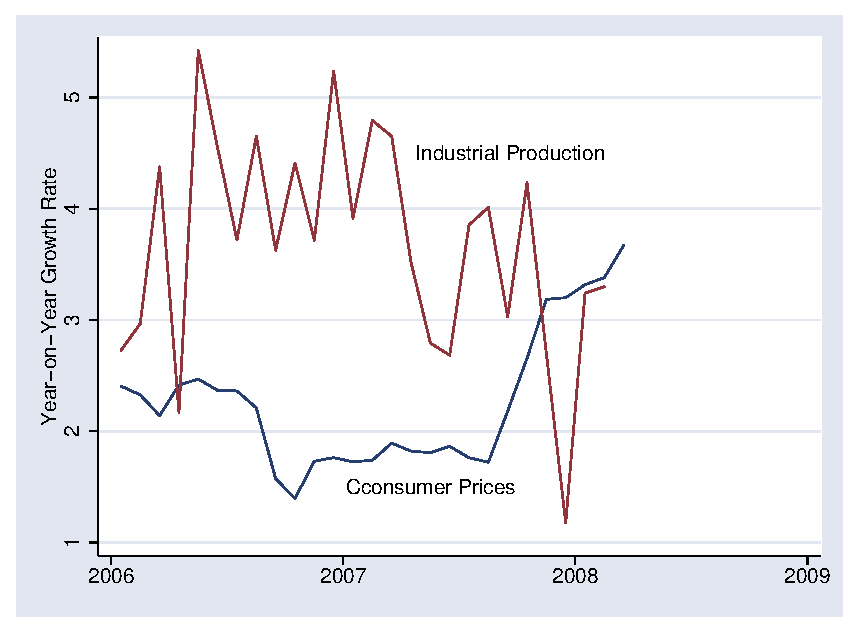
\includegraphics[scale=0.8]{final_08.eps}
    \caption{Growth in prices and industrial production in the 
    Euro Zone.} 
    \label{fig:ez}
\end{figure}


%\begin{comment}
Answer.
\begin{enumerate}
\item Inflation is up sharply, output is flat to down. 

\item The combination in (a) suggests a shift up/left in supply.
Why?  Because output and inflation have moved in opposite directions.
Since supply shocks should be accommodated/reinforced, 
the ECB should raise the short-term interest rate.

\item The ECB's primary mission is stable prices, 
so you should see an increase in interest rates.
This could also be expressed in terms of a Taylor rule, 
possibly with a larger coefficient on inflation 
than output growth.  

\end{enumerate}
%\end{comment}



\end{enumerate}
%\end{comment}


\subsubsection*{Further information}

Similar material is covered in greater depth 
in most macroeconomics textbooks.  
Our favorite is 
%
\begin{itemize}
\item N. Gregory Mankiw, {\it Macroeconomics (6th edition)\/}, ch 9
(10 and 11, too, if you're interested).

%\item Andrew Abel, Ben Bernanke, and Dean Croushore, 
%{\it Macroeconomics (6th edition)\/}, ch 9.
\end{itemize}
%
Any edition will do, but the chapter numbers may vary.  
On measuring potential output, 
here is a range of opinion on the subject:
%
\begin{itemize} 
\item Fed Governor Frederic Mishkin's 
\href{http://www.federalreserve.gov/newsevents/speech/mishkin20070524a.htm}{speech}.

\item Professor Robert Hall's 
\href{http://www.kc.frb.org/publicat/Sympos/2005/PDF/Hall2005.pdf}{critique} or
(better yet) Professor Mankiw's lucid (and short!) 
\href{http://www.kc.frb.org/publicat/Sympos/2005/PDF/Mankiw2005.pdf}{summary and discussion}.  
The essence of Hall's argument is that potential output may very well not be smooth, 
which would contradict most measures of it.
As a practical matter, this would change our view of monetary policy dramatically, 
since many of the movements we see in GDP would be the result of the invisible hand, 
and therefore not something for policymakers to offset. 

\end{itemize}


\vfill \centerline{\it \copyright \ \number\year \ NYU Stern
School of Business}


\end{document} 

OLD STUFF

\subsubsection*{Beyond supply and demand} 


Aggregate supply and demand is 
how most textbooks treat business cycles.
It's also behind much of what you read in the business press.  
But it's not how academic economists think about them.  
The issue is dynamics:  there are no dynamics in the model.
And when you start thinking about dynamics, 
some tricky issues come up that we've ignored ---  
perhaps right so! 
The central one is that current decisions typically depend 
not only on current conditions, but 
on what people expect conditions to be in the future. 
That makes it difficult to determine causality:
did the present cause the future, or the reverse?  


Think about popular comments to the effect that 
consumer demand is driving the economy.
A journalist might say:  high consumer demand led to an economic boom.
The logic is perfectly consistent with our AS/AD analysis, 
but is that really what's going on?  
If we think about consumption, 
one of our first thoughts should be to think about our future income.  
If we expect to have much higher income in the future 
(that MBA is really paying off!), 
we might consume more now.  
But think about what that does to causality:  
for the economy as a whole, has output gone up because we consumed
more, or did we consume more because we expected output to go up? 
It's not easy to tell the difference between the two arguments.  


Investment is similar.  Firms make investment decisions
based on their assessment (ie, guess) 
of market conditions years down the road.  
That's why ``institutions'' are so important:  
good institutions give firms some assurance that the rules won't change 
in ways that make the investment less attractive.  
With respect to business cycles, we could ask the same question 
we asked of consumption:
did high investment lead to a booming economy, 
or did expectations of a booming economy lead to high investment? 
If we're forecasting, we may not care, as long as the two go 
together.
But if we want to understand what's going on, we need to address 
this issue one way or the other.
Fed minutes and analyst reports 
are filled with conjectures over exactly this kind of issue.
 

Sticky wages are another example.  
We noted that output may be below its long-run 
level if the real wage is too high.  
%:  if the wage rate is above where supply equals demand for labor.  
But how was that wage set?  
If workers and firms expect conditions to lead wages to be too high, 
why don't they set a lower wage?  
There may be reasons this could happen anyway, 
but the point is that wages will be based, in part, 
on expected future conditions.  

%All of these examples suggest that the economy is more complicated 
%than the aggregate supply and demand apparatus indicates.  

